\chapter{Background}
\label{cha:backg}

\section{Spectral Clustering}

It is convenient to set a little context, in order to appreciate
better what is the operation that this thesis tries to optimize. For
this we enter a bit into the Spectral Clustering world. In such
context the \gls{Laplacian} Matrix and its second smallest eigenvector
\footnote{This is an abuse of the language of course, when
we say the smallest or biggest eigenvector/eigenpair, we actually refer to
the property of the associated eigenvalue.}
will emerge, and it will become clearer why computing
an eigenvector can serve Data Clustering. The original merit of
finding the value of the \gls{FiedlerVector} goes to Fiedler
\cite{fiedler73}, considered the father of Algebraic Graph Theory. But
the further developments brought by Hagen et al \cite{hagen92} and
Shi et al \cite{shi00}, are closer to the usage seen in our target
application. \\

The stuff we briefly discuss on this chapter could be considered part
of the more theoretical area of Spectral Graph Theory
\cite{brouwer12}. But in more
practical terms, the material exposed here comes mainly from the
standard introductory tutorial to Spectral Clustering by Luxburg \cite{luxburg07},
and from the excellent lecture that Gao gives about the topic on
its Data Mining Course at the University of Buffalo \cite{gao13}.

\subsection{Similarity Graphs}\label{sub:sim-graphs}

If one is doing Data Clustering, one encodes the applications' data
into vectors $\vec{x} \in \R{n}$, but if one is aiming to do Spectral
Clustering we will also need to build an auxiliary graph. This is
because in Spectral Clustering, the operation of computing clusters is
reduced to that of computing graph partitions. To do that, we need to
label our encoded data (vectors) as nodes in an undirected weighted graph $G =
(V,W)$, where the edges' weights will be given by 
a similarity function defined for the problem. This graph is
known as the \emph{Similarity Graph}. \\

Besides the similarity function, which determines the weights on the
graph, there are other sources of variation in the way we connect the
nodes. Below some of the most popular constructions used in Spectral
Clustering, taken from \cite{luxburg07}. \\

\begin{itemize}
  \item The $\epsilon-$neighborhood graph: In this graph we connect a
    couple of nodes $x$ and $y$ only if the value of the similarity
    function is smaller than certain ratio called $\epsilon$. As the
    resulting edges will have values of roughly the same scale, there
    is not much additional information in leaving the weights in this
    graph. \\
  \item The $k-$nearest neighbor graph: In this case a pair of
    vertices $x$ and $y$ will be connected, only if $y$ is among the
    $k-$nearest neighbors of $x$. This construction leads to a
    directed graph, but there are ways to transform it into an
    undirected one (like simply ignoring the direction of the edges, or
    considering mutual neighborhood). \\
  \item The fully connected graph: Here the only requirement for
    connecting a couple of vertices $x$ and $y$ is that their
    similarity function gives a positive value. This type of
    construction usually requires a more sophisticated similarity
    function than a mere euclidean distance, one that does consider
    the local neighborhood of the underlying data. 
\end{itemize}


In the case of this thesis project, the similarity graph was already
given as input data. Therefore, we did not need to deal with the
question of what particular technique to use for its construction. The
details of the similarity function and the graph itself, can not be
disclosed here due patents involved. \\

\subsection{Computing partitions}
Once the \emph{Similarity Graph} is built, the next task in Spectral
Clustering is to use an algorithm to partition it, and from those
partitions to derive the data clusters. This
derivation could be immediate, if we assume that each node in the
\emph{Similarity Graph} represents one vector from our data set.  \\

While Luxburg presents more sophisticated and practical algorithms 
\cite{luxburg07}, we prefer the simpler but more illustrative one
presented by Shi and Malik \cite{shi00}. This is because such
algorithm, allows one to see explicitly how the repetitive computation
of the \gls{FiedlerVector} can produce a complete partition
(clustering). The \cref{alg:rec-2way-cut} shows a template version
of the method, where we can mention the variations related to our work.

\begin{algorithm}
  \label{alg:rec-2way-cut}
  \caption{Recursive 2-way Cut Algorithm}
  %
  \setstretch{1.35}
  \SetKwInOut{Input}{Input}
  \SetKwInOut{Output}{Output}
  \DontPrintSemicolon
  %
  \Input{Similarity matrix and number $k$ of maximum allowed bipartitions (cuts).}
  \BlankLine
  %
  \Output{A partitioned graph, where each partition represents a cluster.}
  \BlankLine
  %
  \textbf{1.} Construct a similarity graph, for example, with one of the
  techniques mentioned in \cref{sub:sim-graphs}.
  \BlankLine
  \BlankLine
  %
  \textbf{2.} Compute the \gls{Laplacian} of the graph. There is more than one
  type of Laplacian, but the one we will use later is the so called
  Unnormalized \gls{Laplacian} (see \cref{sub:lap-fvec}). 
  \BlankLine
  \BlankLine
  %
  \textbf{3.} Compute the second eigenvector (\gls{FiedlerVector}) of the
  \gls{Laplacian}, as it is the one optimizing the chosen
  objective function. The purpose of this function is to seek for well
  balanced partitions, and the most popular choices are Ncut
  \cite{shi00} and RatioCut \cite{hagen92}. We focused on
  RatioCut function in this thesis, as that was the version used by the
  application (see \cref{sub:min-bip-rcut} for further details).
  \BlankLine
  \BlankLine
  %
  \textbf{4.} Using the computed \gls{FiedlerVector} proceed to calculate the
  bi-partition of the \emph{Similarity Graph}. There is more than one
  way of achieving this, and \cite{hagen92} presents several of them
  for the RatioCut function. The one we used in the further sections
  is simply the sign function (see \cref{sub:min-bip-rcut} for further details).
  \BlankLine
  \BlankLine
  %
  \textbf{5.} If the number of cuts has not exceeded the given parameter $k$, and
  if the current partitions need further splitting (according to a
  predefined criteria), then proceed to recursively bi-partition
  the selected pieces.
  \BlankLine
  \BlankLine    
\end{algorithm}
\hfill

Although the general application of Spectral Clustering is to produce
a total partition of the graph, we could consider that the basic
operation is the bi-partition. Given that we can not reveal the actual
algorithm used by our application, let us just say that it also has as a
basic block the bi-partition task. That is why, we focus this
thesis on optimizing such single operation. The
\cref{sub:min-bip-rcut} provides deeper details about it, and
\cref{sub:lap-fvec} explains its relationship with the \gls{FiedlerVector}. 

\subsection{Minimal Bi-Partitional RatioCut}\label{sub:min-bip-rcut}

The work of this thesis lies around the basic operation of
bi-partitioning the similarity graph (removing certain edges such that we
disconnect the vertices set). This is to be done in such way that the
\emph{cut} function $\left(\func{cut}(A,B) = \sum\limits_{\tiny{i \in A
    \ds{,} j \in B}} w_{ij}\right)$ is minimized. This will bring as result
two partitions containing quite similar nodes (according to the similarity
function defined), and then, they could be thought as clusters. The
\cref{fig:min-bip-cut}, adapted from \cite{gao13}, illustrates this
operation.

\begin{figure}[H]
  \centering
  \caption{Minimal Bi-Partitional RatioCut}
  \label{fig:min-bip-cut}  
  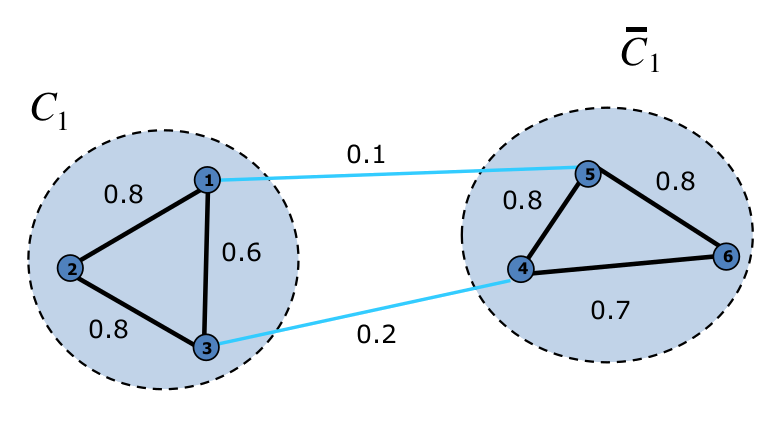
\includegraphics[width=10cm,height=5.5cm]{min-bip-cut-doc}
\end{figure}

The sky blue edges are the minimal \emph{cut} for this example. This results
in two partitions $C_1$ and $\stcomp{C_1}$. While there is more than
one way of formalizing this problem, we care about the one
using the \emph{RatioCut} function (Minimal Bi-Partitional RatioCut Problem),
which favors the solutions containing partitions of roughly
the same size \cref{eq:min-bip-ratio-cut}.

\begin{equation}
  \label{eq:min-bip-ratio-cut}
  \min\limits_{\tiny{C_1 \ds{\subset} V}} \ds{}
  \underbrace{      
    \frac{1}{2}
    \left[
      \dfrac{\func{cut}(C_1,\stcomp{C_1})}{\abs{C_1}} +
      \dfrac{\func{cut}(\stcomp{C_1},C_1)}{\abs{\stcomp{C_1}}}
      \right]
  }_{\func{RatioCut(C_1,\stcomp{C_1})}}
  \ds{\suchthat}
  \func{cut}(A,B) = \sum\limits_{\tiny{i \in A \ds{,} j \in B}} w_{ij}
\end{equation}
\joinbelow{1cm}

Asking for the partitions to have similar sizes, avoids the non
interesting solutions which include singletons\footnote{That is,
  solutions which include a partition with a single node.}, but it also  
makes the optimization problem NP-Hard (see
\cite{wagner93}). This 
is where Spectral Clustering comes to rescue us: By using Linear
Algebra techniques, it can approximate the solutions to the problem
above.

\subsection{The \gls{Laplacian} and its \gls{FiedlerVector}}\label{sub:lap-fvec}
It turns out that if we define the (unnormalized)
\gls{Laplacian} Matrix as $L = D - W$ \footnote{Where $D$ is the diagonal containing
the nodes' degrees and $W$ is the weights matrix of the graph.}, then
the Minimal Bi-Partitional RatioCut Problem reduces to that of minimizing the
Rayleigh-Quotient Function (see
\cref{eq:ratio-cut-min-rayleigh-quo}). The details can be consulted at
\cite{luxburg07} or \cite{gao13}.

\begin{equation}
  \label{eq:ratio-cut-min-rayleigh-quo}
  \min\limits_{C_1 \ds{\subset} V} \func{RatioCut}(C1,\stcomp{C1})
  \ds{\ds{\equiv}}
  \min\limits_{\vec{f} \in \R{n}}
  \underbrace{
    \left(\dfrac{\trans{\vec{f}} L \ds{\vec{f}}}{\trans{\vec{f}} \vec{f}}\right)
  }_{\text{Rayleigh-Quotient}}    
  \ds{\suchthat}
  \vec{f} \in \R{n} \ds{\land} \vec{f} \bot \vec{1}
\end{equation}
\joinbelow{1cm}

The solution given by the vector $\vec{f}$ is an approximation, and it acts
as an indicator function. This means that each one of its cells
represents one node in the graph, and its sign tells whether the
associated node belongs to 
partition $C_1$ or its complement $\stcomp{C_1}$. The property of $f$
being orthogonal to the vector $\vec{1}$, is a consequence of the
\gls{Laplacian} matrix ($L$) properties (see \cite{luxburg07}). \\

Having formulated the problem in terms of the
Rayleigh-Quotient function, allows us to use the immense arsenal that
Linear Algebra has at our disposal. This step is usually skip in
literature, but here we include a more explicit argument. The concrete
theorem that clearly gives a solution to the above problem is the
Courant-Fischer Theorem. In \cref{eq:courant-fischer} we see an
specialized version of such theorem, for the case of the second 
smallest eigenvalue of a real-symmetric matrix $A$ (see \cite{golub13}
for its general formulation).

\begin{equation}
  \label{eq:courant-fischer}
  \lambda_2(A) =
  \max\limits_{\func{dim}(U) = n-1}
  \left[
    \min\limits_{\vec{x} \in U \ds{\land} \norm{\vec{x}} \ne 0}
    \left(  
    \dfrac{\trans{\vec{x}} A \ds{\vec{x}}}{\trans{\vec{x}} \vec{x}}
    \right)
    \right]
\end{equation}
\joinbelow{1cm}

The above result basically tells us that, if we were able to navigate
throughout all the subspaces of dimension $(n-1)$
\footnote{Beware that the formulation of the theorem by Golub in
  \cite{golub13}, may look different on the surface, because it
  mentions that the dimension of the subspaces is $k$ for $\lambda_k$. But
this difference is just cosmetic, because Golub likes to sort the
eigenvalues on descending order, contrary to our convention here
(ascending). Thus for him, $\lambda_2$ is actually
the second biggest eigenvalue. Therefore, the dimension of the
subspaces where we need to search is actually $k$, because $k$ happens
to be $n-1$ for the second smallest eigenvalue in Golub's notation (we
used $n-1$ in the theorem statement due consistency with our ascending
convention for eigenvalues).} 
(where $n$ is the
dimension of the \gls{Laplacian} matrix), then we would know that the answer
to our problem is the eigenvector associated to the second-smallest
eigenvalue of the \gls{Laplacian} (called \gls{FiedlerVector}). The only obstacle
in applying this result, is the non practical task of iterating
over an infinite number of subspaces, but the previously stated
property of $\vec{f} \bot \vec{1}$ solves the problem (see
\cite{luxburg07} for more details about this property). We do not need to
explore all those subspaces, because we know where to look for: in
$\ortc{1}$. This is because the \gls{Laplacian} is known to have $\vec{1}$ as first
eigenvector, and by properties of symmetric matrices, the rest of the
eigenvectors (including the \gls{FiedlerVector}) will need to live on the
orthogonal subspace to \vec{1}. 

\section{The Symmetric Eigenproblem}

The previous sections showed that our Minimal Bi-Partitional RatioCut
Problem can be reduced to minimize the Rayleigh-Quotient function,
which in turn can be solved by computing the \gls{FiedlerVector} of the
\gls{Laplacian} matrix (or in general, to that of computing the second
eigenpair\footnote{By eigenpair we mean a certain eigenvalue and its
  associated eigenvector.}). Our restated problem appears in
\cref{eq:min-rayleigh-quo-snd-eigpair}.

\begin{equation}
  \label{eq:min-rayleigh-quo-snd-eigpair}.  
  \min\limits_{\vec{x} \bot \vec{1} \ds{\land} \norm{\vec{x}} \ne 0}
  \left(  
  \dfrac{\trans{\vec{x}} L \ds{\vec{x}}}{\trans{\vec{x}} \vec{x}}
  \right)
  = \lambda_2
  \suchthat{L\vec{x} = \lambda_2\vec{x}}  
\end{equation}
\joinbelow{1cm}

Before moving on with the algorithm
details of further chapters, this section provides minimal background
theory about such new problem (Symmetric Eigenproblem). Conscious
that this fascinating branch of 
Numerical Linear Algebra is huge, and that we can provide here just a
little taste, we suggest the authoritative references of
\cite{parlett80}, \cite{saad92}, \cite{cullum02}, \cite{demmel97} or
\cite{bai00} for a deeper dive. 

\subsection{The Spectral Theorem}

In dealing with our restated problem, perhaps one of the first things
we should ask ourselves is when it has a solution. For symmetric
matrices like the \gls{Laplacian}, this question has a definite answer given
by the Spectral Theorem (symmetric version):

\begin{theorem}[Spectral Theorem]
\label{the:spec-theorem}
If $A$ is a real symmetric matrix $\implies$ there exists a real orthogonal matrix $Q$ such that $\trans{Q}AQ$ is diagonal. 
\end{theorem}
\joinbelow{1cm}

In the context of \cref{the:spec-theorem}, matrix $Q$ contains the
eigenvectors and matrix $\trans{Q}AQ$ contains the eigenvalues on its
diagonal. There are several proofs of the above theorem, but the one we
recommend for its originality is by Wilf \cite{wilf81}.

\subsection{Numerical Considerations}

Having the guarantee of a theoretical solution does not imply that we
can approximate it numerically without problems. Numerical Analysis,
and in particular Linear Numerical 
Algebra, are immense fields and the amount of context required to grasp
their theory is abundant. But here we just briefly focus on a couple of
aspects that are the bare minimum required, before moving on to the more
practical chapters: We are talking about conditioning and numerical
stability. The information mentioned below was taken from
\cite{bindel09}. \\ 

\subsubsection{Conditioning}
Regardless of the algorithm that we employ to solve the Symmetric
Eigenproblem, is worth to note that the problem itself has a property
called conditioning. In essence, it aims to measure whether small
perturbations on the input will produce small or big perturbations on the
answer (problems are called ill-conditioned if the answer perturbation
is big, and well-conditioned otherwise). For our problem there are two subproblems:
computing eigenvalues and computing eigenvectors \footnote{We
just need the eigenvector, but software routines typically compute both the
eigenvalue and the eigenvector, which we call an eigenpair.}. The
\cref{eq:cond-eigval} and \cref{eq:cond-eigvec} summarize the
conditioning of both subproblems (respectively).

\begin{equation}
  \label{eq:cond-eigval}
  \kappa_{i}(A) = \dfrac{\abs{\lambda_{max}}}{\abs{\lambda_i}}
\end{equation}

\begin{equation}
  \label{eq:cond-eigvec}
  \Delta \vec{v}_i \approx \sum\limits_{\tiny{i \ne j}}
  \dfrac{\trans{\vec{v}_j} \Delta A \vec{v}_i}{\lambda_i - \lambda_j}  
\end{equation}
\joinbelow{1cm}

The \cref{eq:cond-eigval} defines the condition number for each
eigenvalue $\lambda_j$ , and we can see that is a ratio between the maximum
eigenvalue and the one in question. This means that the closer we get
to the maximum (in magnitude), the smallest (better) our condition number will be. On
the other hand, \cref{eq:cond-eigval} describes the perturbation of an
eigenvector $\vec{v}_i$ of $A$ regarding an small perturbation on the
matrix $A$ (called $\Delta A$). We can observe that the perturbation of
$\vec{v}_i$ has a 
contribution from every eigenpair, and the critical part is the
denominator. The closer the eigenvalues are, the bigger the
perturbation will be. \\

The above paragraph basically says that for eigenvalues, we only face
trouble if we target quite small ones, which is not the case for our
particular application \footnote{For our particular matrices, even if
  we compute the
  second smallest eigenvalue, it is still big enough to avoid spikes
  on the condition 
number $\kappa_{2}(A)$.}. But above also says that
eigenvectors could be ill-conditioned even if eigenvalues are not,
which happens when these are clustered (quite close to each
other, and from now on referred as \gls{ClusteredEigenvalues}). This
is a situation we faced in practice for this project, but 
later chapters will mention the workaround that we found for this
scenario (plus the actual, more practical reasons, that we had to avoid
it, see \cref{sub:avoid-clust-eigv}). 

\subsubsection{Numerical Stability}

Numerical Stability is a property of the algorithms we use, and in
short it tells how much additional ``numerical noise'' the computation
adds to the solution (in addition to the perturbation inherent to the
problem conditioning). There is more than one way of formalizing this
notion, but a particularly useful one in Numerical  
Linear Algebra is Backward Numerical Stability. The
\cref{def:backw-stab} is taken from \cite{demmel97}. 

\begin{definition}{Backward Numerical Stability}
  \label{def:backw-stab}
  If $\func{alg}(\vec{x})$ is our algorithm for computing $\func{f}(\vec{x})$,
  including the effects of roundoff, we call $\func{alg}(\vec{x})$ a
  \emph{backward stable algorithm} for $\func{f}(\vec{x})$ if for all
  $\vec{x}$ there is a ``small'' $\Delta x$ such that $\func{alg}(x) =
  \func{f}(\vec{x} + \Delta \vec{x})$. $\Delta x$ is called the
  \emph{backward error}.
\end{definition}

Backward stability means
in essence, that the algorithms compute the exact answer of a very
close problem (in our case $L + \Delta L$). Backward stable algorithms are 
nice, in the sense that they do not add a significant error to the
answer. Thus, they allow us to focus only on the
the perturbations given by the problem conditioning. In our concrete
case of the Symmetric Eigenproblem, and the type of matrices our
application produces, this would reduce to avoiding
\gls{ClusteredEigenvalues}. \\

When we started this thesis, we thought that it was custom to have
formal proofs regarding the overall numerical stability of algorithms,
in particular for the case  of eigensolvers. But for the concrete
algorithms we selected and experimented with, only \gls{MRRR} has 
references to formal proofs about its numerical stability (and not
precisely for the overall algorithm, but for some portions of the
calculations \footnote{Which ultimately makes sense, as the numerical
software is quite complex, built from a lot of subroutines and
layers. In general, it should be easier to discuss numerical stability
at a more granular level, rather than for the whole algorithm.}, see
\cite{dhillon06}). \\   

Above does not mean that \gls{IRLM} or \gls{LOBPCG} do not consider
stability at all. The literature (see \cite{arpack} and
\cite{knyazev01}) does indeed mention concerns, precautions and 
a general focus on achieving this property. Furthermore, all that
work is reflected on the good quality of the results produced (when
comparing against \gls{MRRR}, the gold standard in accuracy). It is just
that, the expectation of finding an explicit proof for the whole
algorithm's stability, does not seem to be a
common practice by Numerical Analysts. We contacted Knyazev
himself, in order to ask about any proof of \gls{LOBPCG}. He
kindly explained that this expectation of the proof was too
high. Therefore, we are happy with claiming that
\gls{IRLM} and \gls{LOBPCG} are stable in a ``practical sense'',
and that the reputation of their authors, along with the good results
seen in experiments, are enough for us to trust them.

